\documentclass[border=12pt]{standalone}
\usepackage[utf8]{inputenc}
\usepackage[dvipsnames,svgnames,x11names]{xcolor}
\usepackage{tikz}
\usetikzlibrary{arrows.meta, positioning, shapes.geometric}
\newcommand{\ryy}{dimension of nothing}
\begin{document}
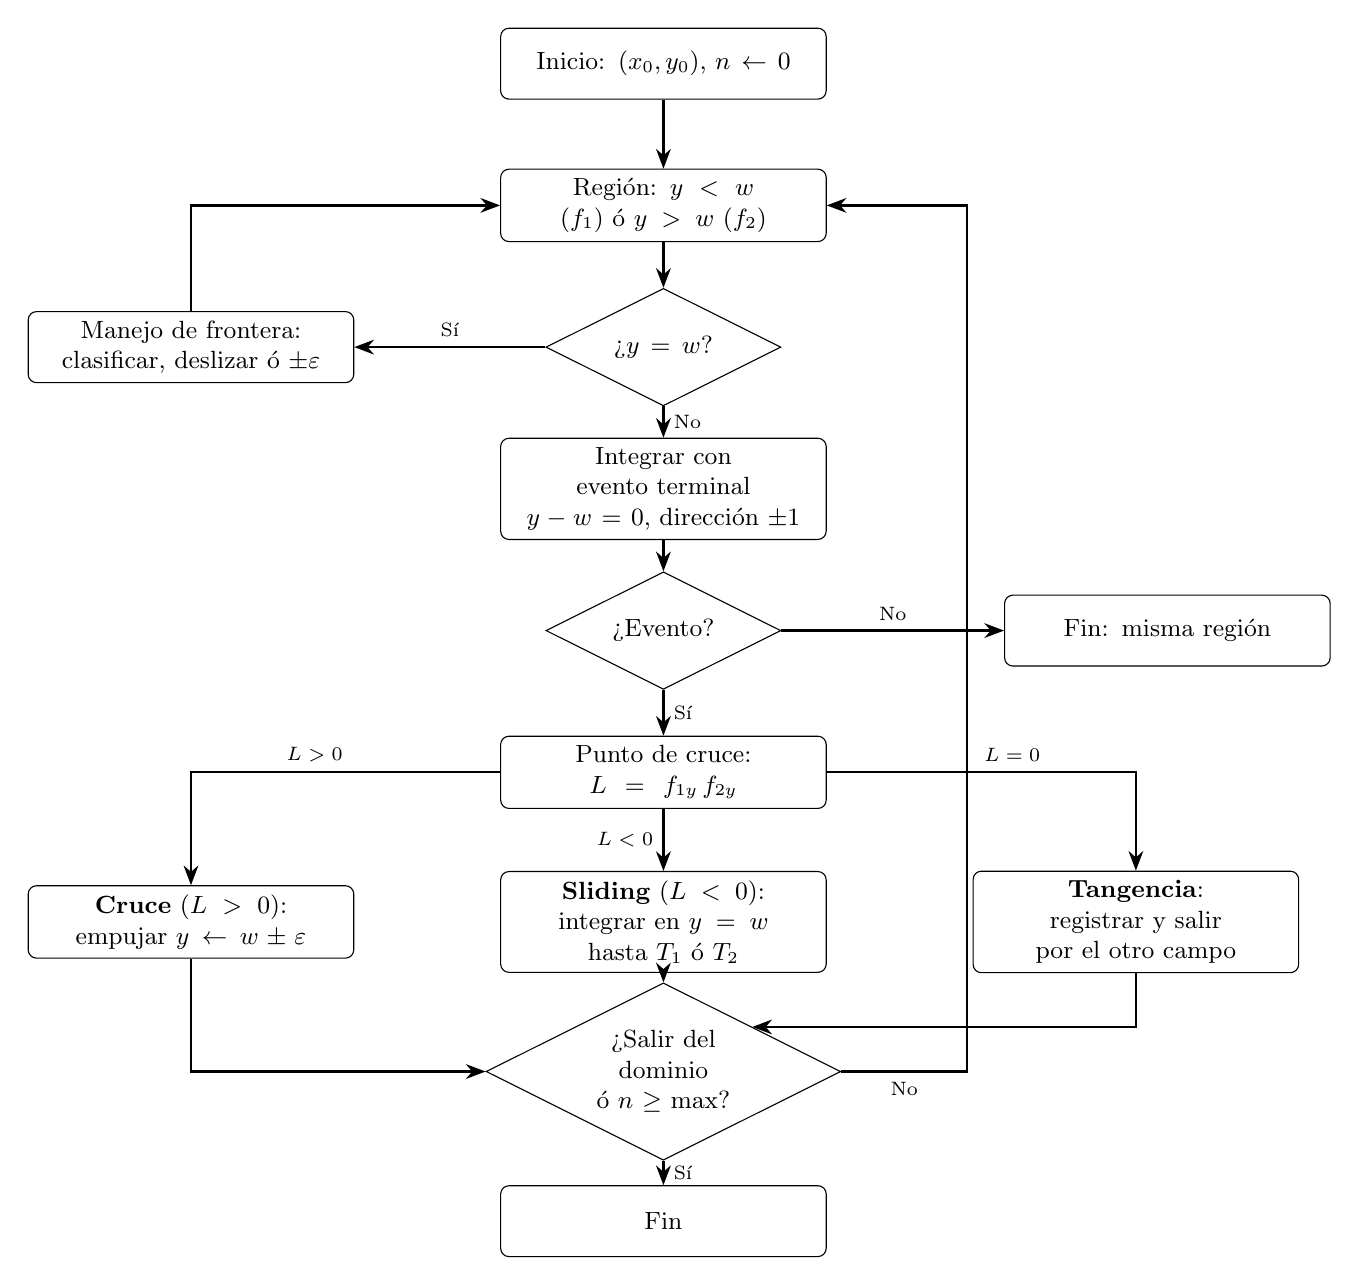
\begin{tikzpicture}[
  p/.style={rectangle, draw, rounded corners=3pt, align=center, text width=3.9cm, minimum height=0.9cm, font=\small},
  d/.style={diamond, draw, align=center, text width=2.0cm, inner sep=2pt, font=\small, aspect=2},
  arr/.style={-{Stealth[length=2.5mm]}, thick},
  lab/.style={font=\scriptsize}
]
  \node[p] (init) at (0,0) {Inicio: $(x_0, y_0)$, $n \gets 0$};
  \node[p] (reg) at (0,-1.8) {Región: $y<w$ ($f_1$) ó $y>w$ ($f_2$)};
  \node[d] (bnd) at (0,-3.6) {¿$y=w$?};
  \node[p] (bproc) at (-6.0,-3.6) {Manejo de frontera:\\clasificar, deslizar ó $\pm\varepsilon$};
  \node[p] (inte) at (0,-5.4) {Integrar con evento terminal\\$y-w=0$, dirección $\pm 1$};
  \node[d] (evh) at (0,-7.2) {¿Evento?};
  \node[p] (finc) at (6.4,-7.2) {Fin: misma región};
  \node[p] (clas) at (0,-9.0) {Punto de cruce:\\$L = f_{1y}\,f_{2y}$};
  \node[p] (cr) at (-6.0,-10.9) {\textbf{Cruce} ($L>0$):\\empujar $y \leftarrow w \pm \varepsilon$};
  \node[p] (sl) at (0,-10.9) {\textbf{Sliding} ($L<0$):\\integrar en $y=w$ hasta $T_1$ ó $T_2$};
  \node[p] (tn) at (6.0,-10.9) {\textbf{Tangencia}:\\registrar y salir por el otro campo};
  \node[d] (chk) at (0,-12.8) {¿Salir del dominio\\ó $n\ge$ max?};
  \node[p] (fin) at (0,-14.7) {Fin};
  \draw[arr] (init.south) -- (reg.north);
  \draw[arr] (reg.south) -- (bnd.north);
  \draw[arr] (bnd.west) -- node[lab,above]{Sí} (bproc.east);
  \draw[arr] (bnd.south) -- node[lab,right]{No} (inte.north);
  \draw[arr] (inte.south) -- (evh.north);
  \draw[arr] (evh.east) -- node[lab,above]{No} (finc.west);
  \draw[arr] (evh.south) -- node[lab,right]{Sí} (clas.north);
  \draw[arr] (clas.west) -| node[lab,above,pos=0.3]{$L>0$} (cr.north);
  \draw[arr] (clas.south) -- node[lab,left]{$L<0$} (sl.north);
  \draw[arr] (clas.east) -| node[lab,above,pos=0.3]{$L=0$} (tn.north);
  \draw[arr] (cr.south) |- (chk.west);
  \draw[arr] (sl.south) -- (chk.north);
  \draw[arr] (tn.south) |- (chk.north east);
  \draw[arr] (bproc.north) |- (reg.west);
  \draw[arr] (chk.south) -- node[lab,right]{Sí} (fin.north);
  \draw[arr] (chk.east) -- node[lab,below]{No} ++(1.6,0) |- (reg.east);
\end{tikzpicture}
\end{document}